\section{CFPQ on planar digraphs}

\subsection{Dynamic transitive closure}

We want to consider algorithms for semi-dynamic transitive closure for the case of a planar graph. Our algorithm needs to support only edge insertions that do not violate planarity.

There are several algorithms that look into the problem of dynamic reachability in planar digraphs and have sublinear both update and query time~\cite{10.5555/647903.739284},~\cite{karczmarz2018data},~\cite{kao2008encyclopedia}. 

Some algorithms~\cite{10.5555/1778580.1778635},~\cite{karczmarz2018data} restrict insertions to only that edges that respect the specific embedding of the planar graph. 

\todo[inline]{maybe we can choose one embedding at random and hope that nothing will violate it. So it will be monte-carlo (why it will have good probability? where from can we get all the possible non-isomorphic embeddings?)}  

The algorithms that allow edge insertions not with respect to the embedding of the graph, but to the planarity, are described in~\cite{10.5555/647903.739284},~\cite{10.1145/300515.300517}. The main idea of both articles is the same: a planar graph is separated into \textit{clusters} (edge induced subgraphs) for which reachability is shown by their sparse substitute $S$. \textit{Sparse substitute} is a graph that contains the reachability information between some set of vertices that lie in the same face of an embedded graph.

We show the results of~\cite{10.5555/647903.739284} more closely as they differ from the results of~\cite{10.1145/300515.300517} only by a logarithmic factor, have the same idea and are easier for understanding. 

Updates and queries are the following: adding or deleting the edge between vertices $u, v$, checking reachability, checking if new edge $(u, v)$ violates planarity. 

Every update procedure modifies a constant number of clusters, for which we reconstruct their sparse substitutes. If the procedure added the edge, new edge forms its own cluster. Moreover after every $\mathcal{O}(n^{1/3})$ insertions we rebuild cluster partition and sparse substitutes from the scratch so that clusters do not lose their properties, this rebuilding time is distributed between these $\mathcal{O}(n^{1/3})$ insertions, so insertion time is amortized. 

After splitting graph into clusters and looking into its sparse substitute update or query about vertices $u, v$ can be done by placing clusters of the vertices $u, v$ in the original graph $G$ into the graph of sparse substitutes $S$.

For maintaining dynamic transitive closure in this way we only need planarity to divide graph $G$ into clusters and for each cluster to build its sparse substitute. As we rebuild cluster partition and substitutes at the beginning and after every $\mathcal{O}(n^{\frac{1}{3}})$ edge-insertions, graph needs to remain planar during the updates. 

The results are the following.
 
\begin{enumerate}
	\item The amount of time for preprocessing is $\mathcal{O}(n \log n)$ --- in this time we find the separation of the given graph $G$ into $\mathcal{O}(n^{\frac{1}{3}})$ clusters (each consists of no more than $n^{\frac{2}{3}}$ edges of $G$) and build sparse substitution graph $S$ of total size $\mathcal{O}(n^{\frac{2}{3}} \log n)$ for them.
	
	\item After that we can perform add operation in $\mathcal{O}(n^{\frac{2}{3}} \log n)$ amortized time, delete operation in $\mathcal{O}(n^{\frac{2}{3}} \log n)$ worst-case time.
	
	\item Reachability query takes $\mathcal{O}(n^{\frac{2}{3}} \log n)$ worst-case time.
	
	\item Checking if the graph is planar can be done in $\mathcal{O}(n^{\frac{1}{2}})$ amortized time. 
\end{enumerate}

Let us look closely on how can we use the power of sparse substitution on our incremental transitive closure problem.

\begin{proposition}
We can maintain the structure described in~\cite{10.5555/647903.739284} not only for planar graphs, but for planar graphs with $\mathcal{O}(n^{\frac{1}{3}})$ edges that violate planarity. 
\end{proposition}

$\square$
In~\cite{10.5555/647903.739284} the number of clusters is $\mathcal{O}(n^{\frac{1}{3}})$. In the beginning and after every $\mathcal{O}(n^{\frac{1}{3}})$ edge insertions we rebuild sparse substitute graph $S$. and in these moments we need planarity. We can additionally maintain the set of non-planar edges, each edge of this set will present its own cluster and will not take part in the rebuilding of sparse substitution. Edge is \textit{non-planar} if its insertion to current planar graph $G$ makes it non-planar.
$\hfill\blacksquare$

\begin{proposition}
We can add edges in the graph and print out new pairs of reachable vertices for every insertion in $\mathcal{O}(n^{\frac{5}{3}})$ total time for every sequence of insertions if our model allows parallel computations.
\end{proposition}

$\square$
From~\cite{10.5555/647903.739284} we can add an edge $(u, v)$ in $\mathcal{O}(n^{\frac{2}{3}}\log n)$ amortized time. We want to get all pairs of vertices that are connected through the new edge.

We can run DFS from $v$ and DFS on reversed edges from $u$ in graph $S$ of sparse substitutes. DFS runs in time proportional to the size of the graph $S$ --- $\mathcal{O}(n^{\frac{2}{3}} \log n)$. After that for every cluster in the original graph $G$ we create dummy vertex $s$ and edges from $s$ to all boundary vertices in the cluster that were reached from $u$ and $v$ respectively. Then run DFS from this dummy vertex $s$. We print out every vertex that was reached by our DFSs, so we get two lists $U$ and $V$ for beginnings and the endings of the paths, going through $(u, v)$.

If any vertex $w$ is reachable from $v$ (without loss of generation), then it is a boundary vertex or lie in some cluster and is reachable from some boundary vertex of this cluster. In both cases, one of DFS's will print it out and the algorithm is correct. 

If we can run these DFS's in parallel (there are $\mathcal{O}(n^{\frac{1}{3}})$ clusters and the same number of DFS's), then each of them will take $\mathcal{O}(n^{\frac{2}{3}})$ amount of time (all cluster have $\mathcal{O}(n^{\frac{2}{3}})$ edges by definition in~\cite{10.5555/647903.739284}). As maximum number of edges in the planar graph is linear, the total amount of time will be $\mathcal{O}(n^{\frac{5}{3}})$ for every sequence of edge insertions.
$\hfill\blacksquare$

\begin{conjecture}
If our model does not allow parallel computations total amount of time for every sequence of insertions is at most $\mathcal{O}(n^2)$ and planarity does not get us any advantage in solving the problem of dynamic reachability (in amortized time per edge and query).
\end{conjecture}

[Thoughts]
If our model can not run algorithms in parallel, then the amount of time taken by iterating DFS's described above for every cluster is linear --- $\mathcal{O}(n)$. This means that usual DFS on the original graph $G$ has the same complexity and we will spend in total $\mathcal{O}(n^2)$ time.
$\hfill\blacksquare$

\todo[inline]{maybe we can spare some space ($\mathcal{O}(n^2)$?) so we can store list of reachable vertices from any boundary vertex and somehow update them during the edge additions?}

\todo[inline]{is there a way to apply this to graphs with fixed thickness? if yes, finding book-thickness is NP-hard in general case but we can restrict maximal vertex degree to get constant thickness. For grammars with $O(1)$ rule length (for example, in Chomsky normal form) and planar graphs we get planar subgraph splitting of the product directly. Is there a way to find this splitting for the given graph $G$ if we have bounding constant on degrees of its vertices?}

\todo[inline]{for planar graphs and short production rules: number of clusters defined by $c$ partitions are no more than $n^{\frac{1}{3} \cdot c}$? maybe play with constants to apply structure of the article to  graphs with thickness=2 (planar x n. Ch. form)}

\subsection{Planarity of Kronecker product of digraphs with labels}

\paragraph{Planarity of Kronecker product}

From results of~\cite{farzan1977kronecker} we know criteria for planarity of Kronecker product of two graphs:

\begin{theorem}[~\citep{farzan1977kronecker}]
\label{theorem:farzan}
Let $G_1$ and $G_2$ be connected graphs with more than four vertices.
Then $G_1 \wedge G_2$ is planar if and only if either:
\begin{enumerate}
	\item[(i)] one of the graphs is a path and the other one is 1-contractible to a path or a circuit, or
	\item[(ii)] one of them is a circuit and the other is 1-contractible to a path.
\end{enumerate}
\end{theorem}

A 1-contraction of $G$ is the removal from $G$ of each vertex of
degree 1 (and its incident edge).


\begin{figure}[h]

  \begin{center}  
  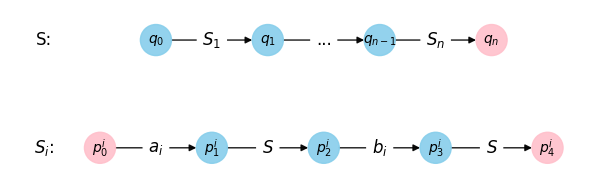
\includegraphics[scale = 0.4]{dyck_n.png}
  \end{center}

  \caption{Possible RSM for Dyck language on $n$ types of brackets. Red vertices $q_n, p^i_4 \; \forall i \in \{1, \ldots, n\}$  are final states, $q_0, p^i_0 \; \forall i \in \{1, \ldots, n\}$ are initial states in each box}

  \label{fig:dyck_n}

\end{figure}

\begin{corollary}
\label{cor:path_circuit}
If we fix the input grammar to grammar of Dyck language, then planarity of the Kronecker product is guaranteed if input graph is 1-contractible to a path or is a circuit.
\end{corollary}

\paragraph{Necessary conditions for planarity of Kronecker product of digraphs}

Let us consider the case of product of two planar digraphs. From~\citep{farzan1977kronecker} it is known, that Kronecker product of $K_{1, 3}$ with itself if non-planar.

\begin{proposition}
If $G_1$ and $G_2$ contain subraphs $K_{1, 3}$ oriented as in Fig.~\ref{fig:k13_0},~\ref{fig:k13_3},~\ref{fig:k13_12} or~\ref{fig:k13_21}, then their Kronecker product is non-planar. 
\end{proposition}

$\square$
Proof is a brute-force algorithm that checks planarity of Kronecker product for all possible orientations of pairs of graphs $K_{1, 3}$.

If graphs $G_1$ and $G_2$ contain pair of subgraphs $K_{1, 3}$ which Kronecker product is non-planar, then $G_1 \wedge G_2$ is non-planar too.
$\hfill\blacksquare$

\begin{figure}[h]

  \begin{center}  
  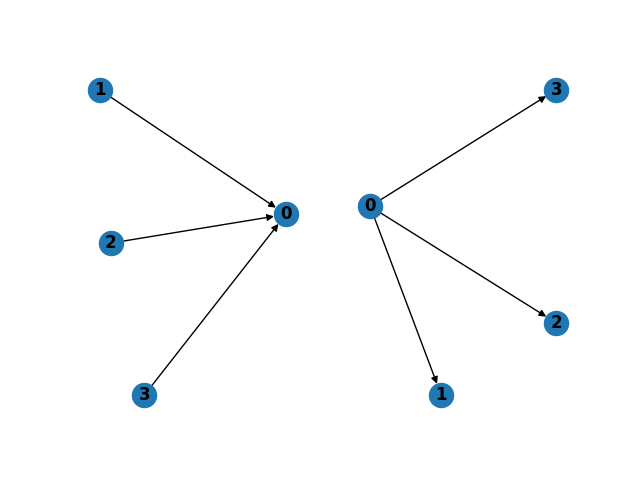
\includegraphics[scale = 0.3]{k13_0.png}
  \end{center}

  \caption{Orientation of the edges of $K_{1, 3}$ graphs, which Kronecker product is non-planar: all edges of the graph at the right are oriented from vertex $0$}

  \label{fig:k13_0}

\end{figure}


\begin{figure}[h]

  \begin{center}  
  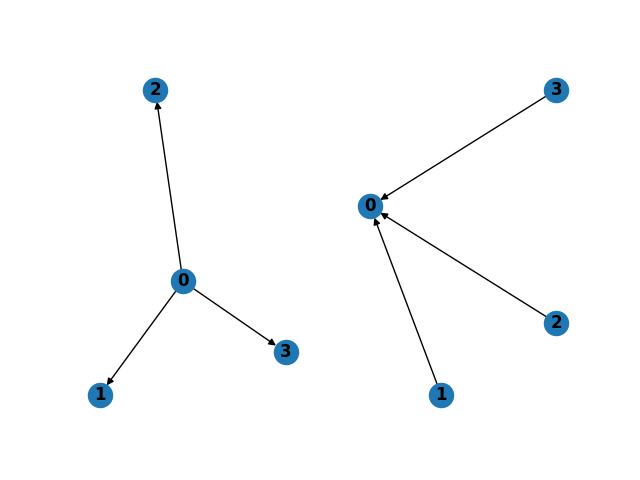
\includegraphics[scale = 0.3]{k13_3.png}
  \end{center}

  \caption{Orientation of the edges of $K_{1, 3}$ graphs, which Kronecker product is non-planar: all edges of the right graph are oriented to vertex $0$}

  \label{fig:k13_3}

\end{figure}

\begin{figure}[h]

  \begin{center}  
  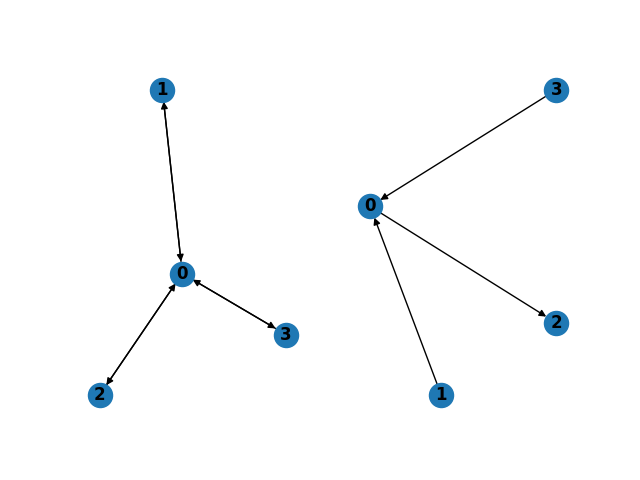
\includegraphics[scale = 0.3]{k13_12.png}
  \end{center}

  \caption{Orientation of the edges of $K_{1, 3}$ graphs, which Kronecker product is non-planar: edges of the right graph are oriented 2 to vertex $0$ and 1 from it}

  \label{fig:k13_12}

\end{figure}

\begin{figure}[h]

  \begin{center}  
  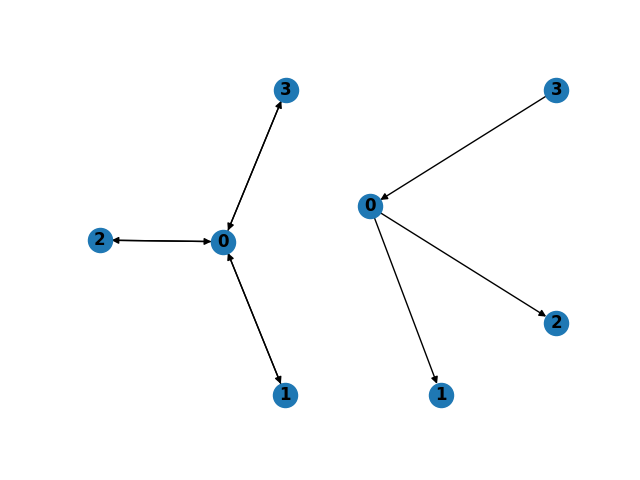
\includegraphics[scale = 0.3]{k13_21.png}
  \end{center}

  \caption{Orientation of the edges of $K_{1, 3}$ graphs, which Kronecker product is non-planar: edges of the right graph are oriented 1 to vertex $0$ and 2 from it}

  \label{fig:k13_21}

\end{figure}

\paragraph{Sufficient conditions for planarity of Kronecker product of digraphs}

Let $G_S$ be a subgraph of the input graph $G$ consisting of the edges that are labelled with $S$ symbol (terminal or non-terminal).

\todo[inline]{let grammar be in Chomsky normal form. then for every rule $S \rightarrow AB$ we need not only outerplanarity for subgraph $G_A \wedge A$ and $G_B \wedge B$, but fixed-order-book-thickness = 1 for some order of vertices of $G$ (because $G_A \wedge -A\rightarrow$ and $G_B \wedge -B\rightarrow$ are sharing $|G|$ vertices)}

\todo[inline]{maybe ordered-book-thickness can be reduced to partitioned-T-coherent 2-page book embedding?}

\todo[inline]{any chance to bound crossing number to $O(n^{\frac{1}{3}})$ in simultaneous embedding?}

\paragraph{Decomposition of the graph into planar layers}

Suppose we have grammar RSM graph in form of paths (for example, in Chomsky normal form or as in Fig.~\ref{fig:dyck_n}). By the Cor.~\ref{cor:path_circuit} we can decompose Kronecker product graph into planar layers by decomposing the input graph into paths and circuits.

\todo[inline]{how to get reachability between the different layers?}

\todo[inline]{clusters in dynamic structure are built based on embedding (triangulated, then divided). Embeddings for different layers may be different, meaning that most likely we can't take the same clusters in every layer to get the same structure and easy reachability}

It is known~\cite{lovasz1968covering} that every graph can be decomposed into $\mathcal{O}(n)$ paths and circuits and there are examples where at least $\frac{n}{2}$ paths are needed.

\begin{theorem}~\cite{lovasz1968covering}
A graph of $n$ vertices can be covered by $\leq \left[ \frac{n}{2} \right]$ disjoint paths and circuits.
\end{theorem}

The decomposition is built by induction on $\lambda(G) = 2 \cdot \mathcal{E}(G) - \sigma(G)$, where $\mathcal{E}(G)$ is the number of edges in graph $G$ and $\delta(G)$ is the number of non-isolated vertices. In every step of induction $\frac{n}{2}$ paths can be rebuilt in worst case. 

\todo[inline]{any chance to built it in less than $\mathcal{O}(n^3)$? if yes, can we afford rebuilding it once in $\mathcal{O}(n^{\frac{2}{3}})$ insertions?}

Inserting a new edge between two vertices at least one of which has odd degree is easy. We store in every vertex $v$ pointers to all paths $P_v^1, \ldots, P_v^k$ that end in it. We can continue one of that paths $P$ in $\mathcal{O}(1)$ by the new edge $(v, u)$ by deleting pointer to $P$ from $v$, adding pointer to $u$ and adding the edge $(u, v)$ to $P$. In case when $2 \nmid deg(v)$ at least one path should end in $v$ and that $P$ is continued.

\todo[inline]{is there an easy way to change to decomposition in case when both vertices at the end of the edge have even degree? Looks like not, because if there are only paths nearby these vertices, then we add two new vertices of odd degree, meaning that they too should be the end of some path. Can we always find a vertex with circuit nearby? if yes, how to change circuit to a path in a fast way?}

\textit{notes:}

Suppose we have a grammar in Chomsky normal form.

By the path-form of the grammar, we know that edges in Kronecker product graph are directed from left to the right (as are in path from grammar). By the definition of CFPQ algorithm, we know that new edge $\overrightarrow{(v, u)}$ is added so that it forms a triangle with some of the existing ones $\overrightarrow{(v, w)},\overrightarrow{(w, u)}$. Then we can continue some path if $2 \nmid outdeg(v)$ or $2 \nmid indeg(u)$ because only outgoing edges of $v$ and only ingoing edges of $u$ are present in Kronecker product graph as path of grammar consists of exactly two edges.

\todo[inline]{what to do with the other edges added to Kronecker product graph formed from new edge in input graph? for them there is no such triangular property} 

\paragraph{My useful articles}

A note on outerplanarity:~\cite{jha1993note}

About book thickness:~\cite{bernhart1979book}

Ordered book thickness:~\cite{10.1007/978-3-030-59267-7_35}

(Ordered) Book thickness in terms of vertex cover:~\cite{bhore2019parameterized}

Crossing number in simultaneous embedding:~\cite{crossing2009}

Simultaneous embedding of planar and outerplanar graphs on a grid:~\cite{brass2007simultaneous}


